\chapter{ABC}

This chapter will outline a series of illustrative ABC examples. These will serve to demonstrate core concepts touched on in the introduction, demonstrate ABC can sample from complex distributions, and develop the boutique code base which form the foundations of this project. The code for the examples in this section can be found at \url{https://github.com/tomconnell/dram}.\\

\section{Toy problem 1: 1D Gaussian}
As a simple first example consider we have observed $n = 100$ realizations from the Gaussian model $\bm{g_s}(\bm{\theta}) = \frac{1}{\sqrt{2\pi\sigma^2}}\ \text{exp}\Big[\frac{-\mu^2}{2\sigma^2}\Big]$. Our unknown model parameters are $\bm{\theta} = [\mu,\sigma]$. Given we have access to simulation from this model it is possible to leverage ABC algorithms to estimate these unknown model parameters. A synthetic dataset for this problem is created with $\mu = 5$ and $\sigma = 2$. The summary statistics sample mean, $\bar{\mu}$, and sample standard deviation, $\bar{\sigma}$, are used. These provide sufficient statistics with a 1:1 correspondance to the unknown parameters. Figure \ref{toy1-fig1} plots the ABC posterior obtained from using algorithm \ref{ABCrejectionsampler}, the traditional form of an ABC rejection sampler, compared to the analytical likelihood. The metric over summary statistics is evaluated marginally and hence takes the form $\rho = |S_1(\bm{y^*}) - S_1(\bm{y})| +| S_2(\bm{y^*}) - S_2(\bm{y})|$. A uniform prior is used to give equal probability to a bounded area, $p(\mu) = \mathcal{U}(0,10)$ and $p(\sigma) = \mathcal{U}(0,10)$. 
Figure \ref{toy1-fig2} explores the impact of varying the tolerance for this problem.\\

\begin{figure}[H]
	\centering
	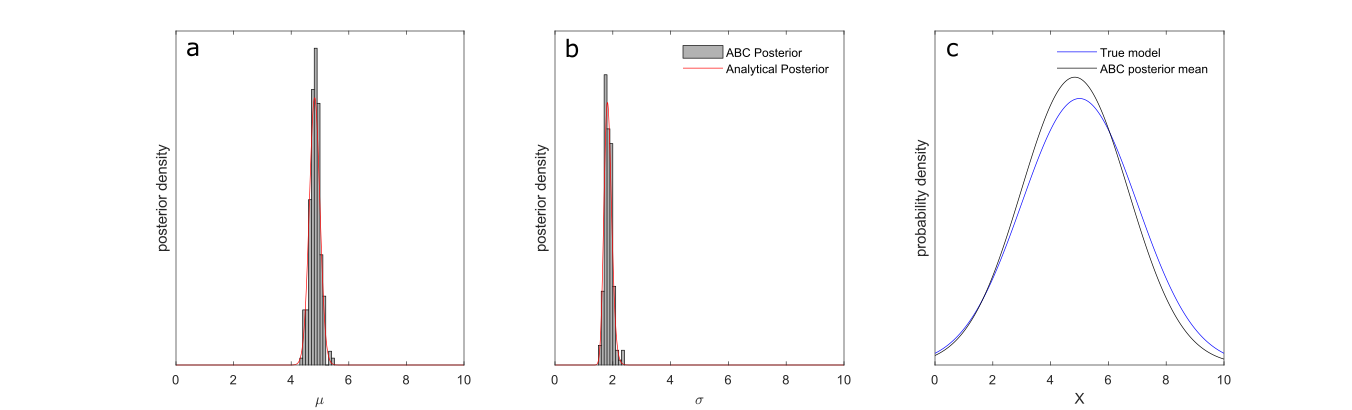
\includegraphics[scale=0.45]{toy1-fig1}
	\caption{Posterior comparison between ABC and traditional likelihood inference for estimating the parameters, $\bm{\theta} = [\mu,\sigma]$, to a Gaussian model given $n = 100$ observations, $\bm{y}$. The ABC algorithm, algorithm \ref{ABCrejectionsampler}, uses 1 million repititions and a tolerance $\epsilon = 0.1$. The likelihood takes the form $\mathcal{L}(\bm{\theta}|\bm{Y}) = (2\pi\sigma^2)^{-n/2}\ \text{exp}\big[-\frac{1}{2\sigma^2}\sum_{i = 1}^{n}(y_i-\mu)^2\big]$. (a) Marginal posterior compared to marginal ABC posterior for unknown parameter $\mu$. (b) same as (a) but for unknown parameter $\sigma$. (c) Mean ABC posterior model compared to true model.}
	\label{toy1-fig1}
\end{figure}

\begin{figure}[H]
	\centering
	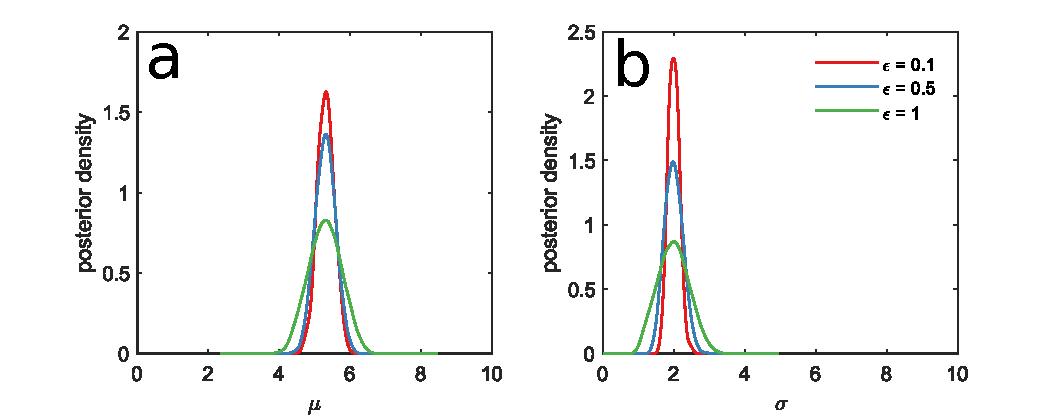
\includegraphics[scale=0.6]{toy1-fig2}
	\caption{The effect of varying the tolerance $\epsilon$ when estimating $\bm{\theta} = [\mu,\sigma]$ to a Gaussian model given given $n = 100$ observations, $\bm{y}$. Three tolerances are considered, $\epsilon = 0.1$, $\epsilon = 1$, $\epsilon = 5$. (a) Marginal ABC posterior for unknown parameter $\mu$. The true value is $\mu = 5$ (b) same as (a) but for unknown parameter $\sigma$. The true value is $\sigma = 2$}.
	\label{toy1-fig2}
\end{figure}

Figure \ref{toy1-fig1} demonstrates that with sufficient statistics and a low tolerance ABC can accurately resolve the posterior using only the ability to simulate data. However, as figure \ref{toy1-fig2}, demonstrates, with a high tolerance significant bias is introduced into the posterior and uncertainty is significantly over-estimated. It is true that increasing increasing the tolerance increases the acceptance rate and hence relaxes computational resources. In this case the acceptance rate with $\epsilon = 0.1$ was $X$, while the acceptance rate with $\epsilon = 5$ was $Y$. Under a model which is expensive to simulate from walking the tightrope between accuracy and efficiency becomes important and needs to be carefully examined. 

\section{Toy problem 2: Linear regression}




\section{Toy problem 3: Bivariate Gaussian}




\section{Toy problem 4: Banana distribution}



 